\chapter*{Auroville\markboth{Auroville}{}}
\section*{13 décembre 2015}
A 10km de Pondichéry, Auroville est une cité expérimentale d'environ 2000 habitants créée en 1968. Des gens de tous les pays y testent de nouvelles façons de vivre, de travailler, d'apprendre tout en cherchant un développement spirituel. 

 Je retrouve Xavier que j'avais rencontré il y a 2 ans en France. Depuis, il s'est installé ici avec sa famille pour devenir aurovillien. 
\begin{center} 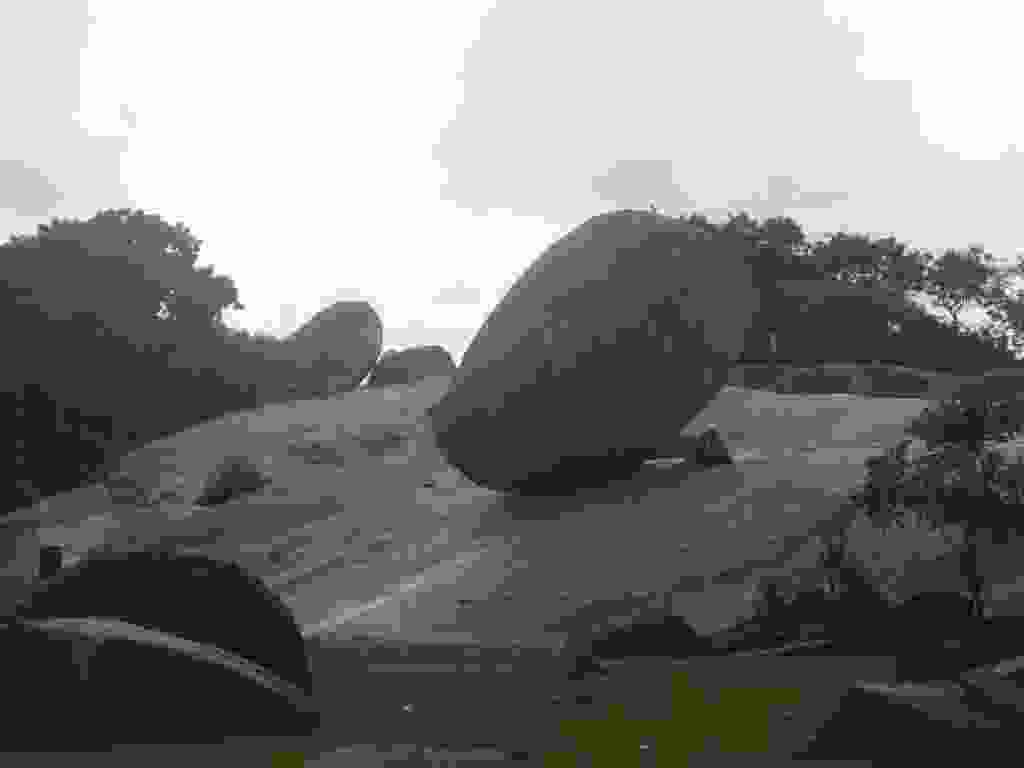
\includegraphics[width=\mywidth]{../wp-content/uploads/2015/12/wpid-oi000594-1024x768.jpg} \end{center}

\pagebreak
 Matrimandir, symbole spirituel au centre de la cité, il y a des pièces pour la méditation dedans. 
\begin{center} 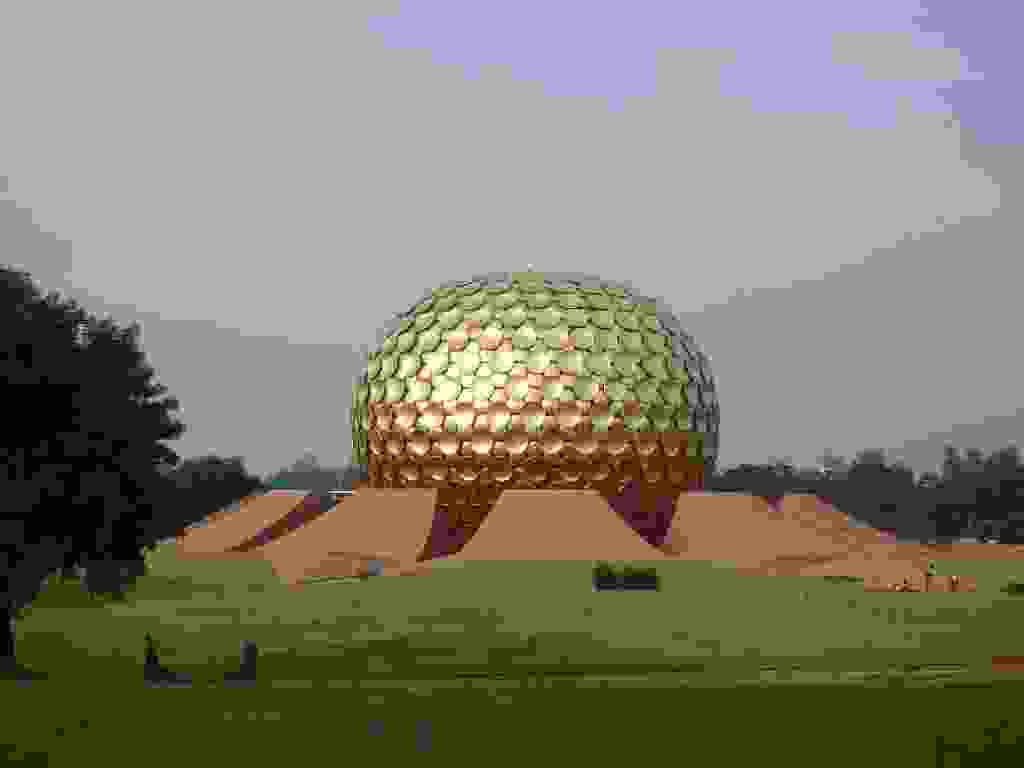
\includegraphics[width=\mywidth]{../wp-content/uploads/2015/12/wpid-oi000633-1024x768.jpg} \end{center}

 Auroville est constituée de dizaines de communautés avec chacune une organisation et un projet particulier.

 Je reste 1 semaine comme volontaire au Youth Center. 
\begin{center} 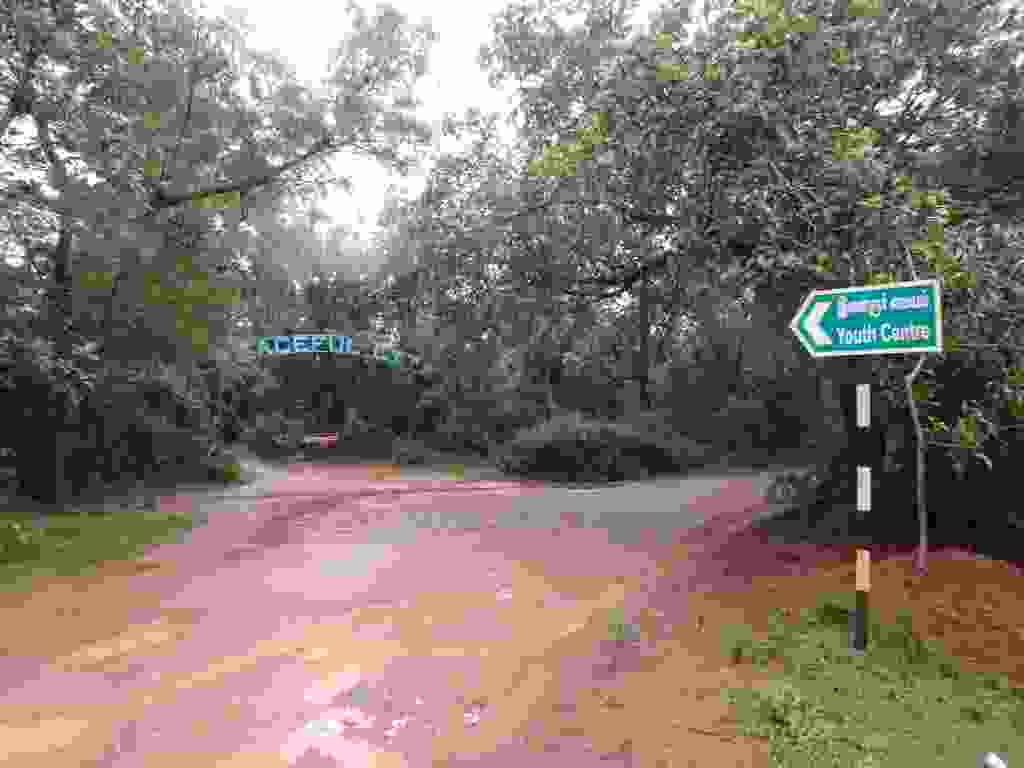
\includegraphics[width=\mywidth]{../wp-content/uploads/2015/12/wpid-oi000558-1024x768.jpg} \end{center}
\begin{center} 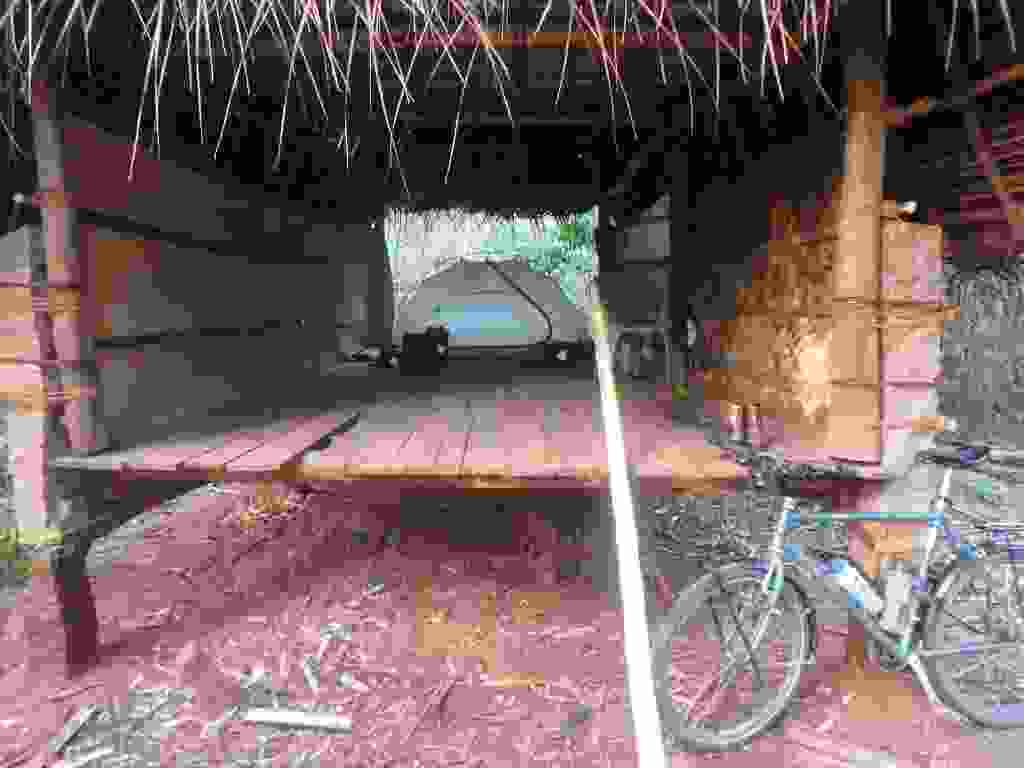
\includegraphics[width=\mywidth]{../wp-content/uploads/2015/12/wpid-oi0006011-1024x768.jpg} \end{center}

 6 jeunes vivent ici en permanence dans des cabanes dans les arbres. 
\begin{center} 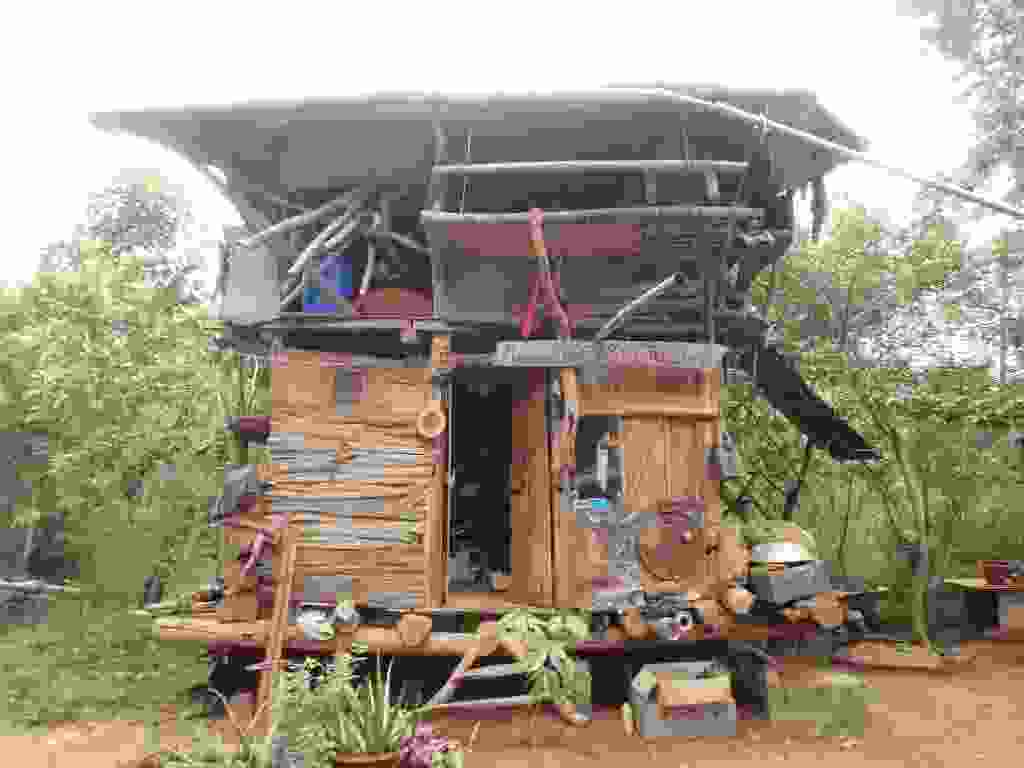
\includegraphics[width=\mywidth]{../wp-content/uploads/2015/12/wpid-oi000607-1024x768.jpg} \end{center}
\begin{center} 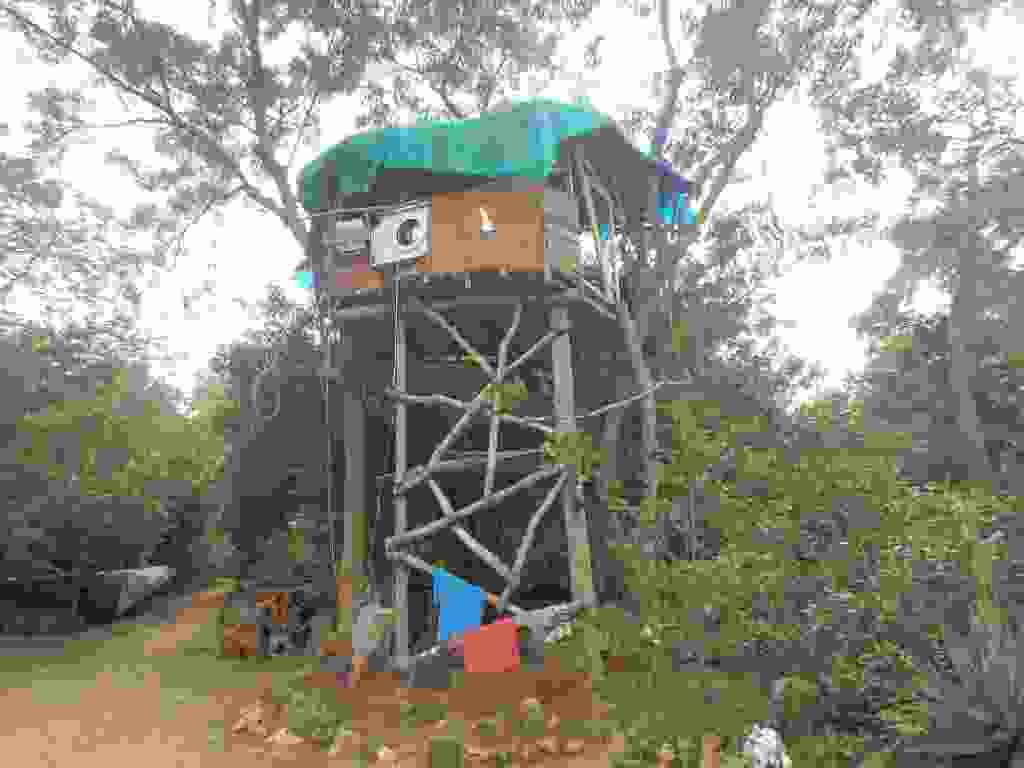
\includegraphics[width=\mywidth]{../wp-content/uploads/2015/12/wpid-oi000630-1024x768.jpg} \end{center}
\begin{center} 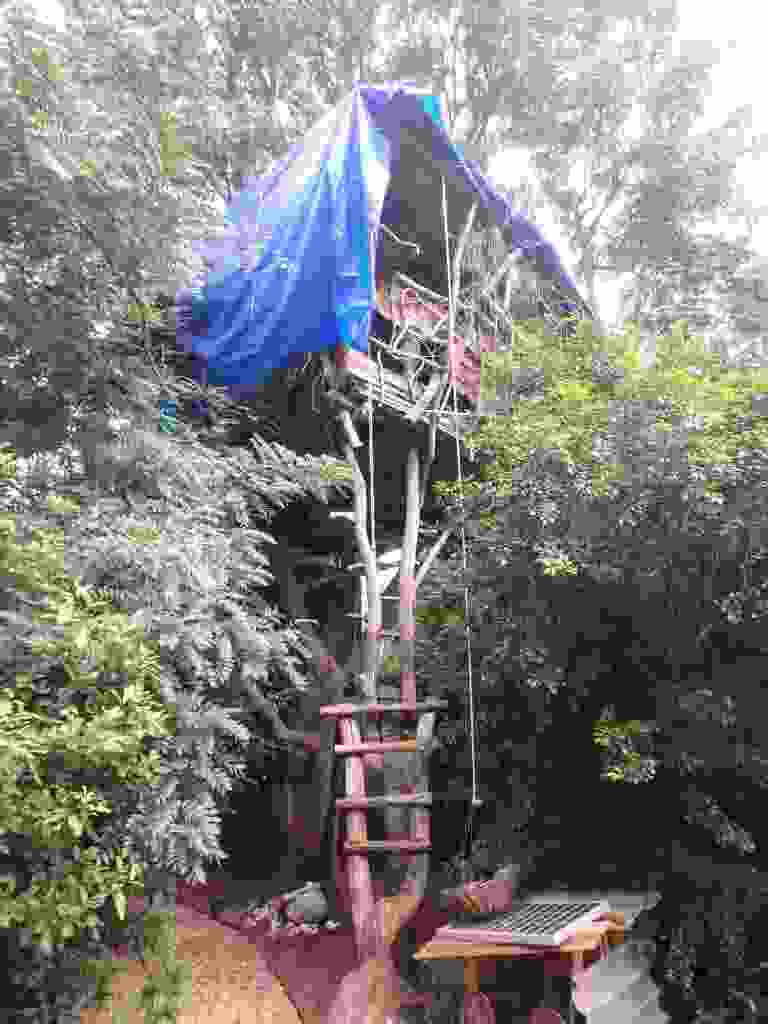
\includegraphics[height=\mywidth]{../wp-content/uploads/2015/12/wpid-oi000631-e1449574701965-768x1024.jpg} \end{center}
 \begin{center} 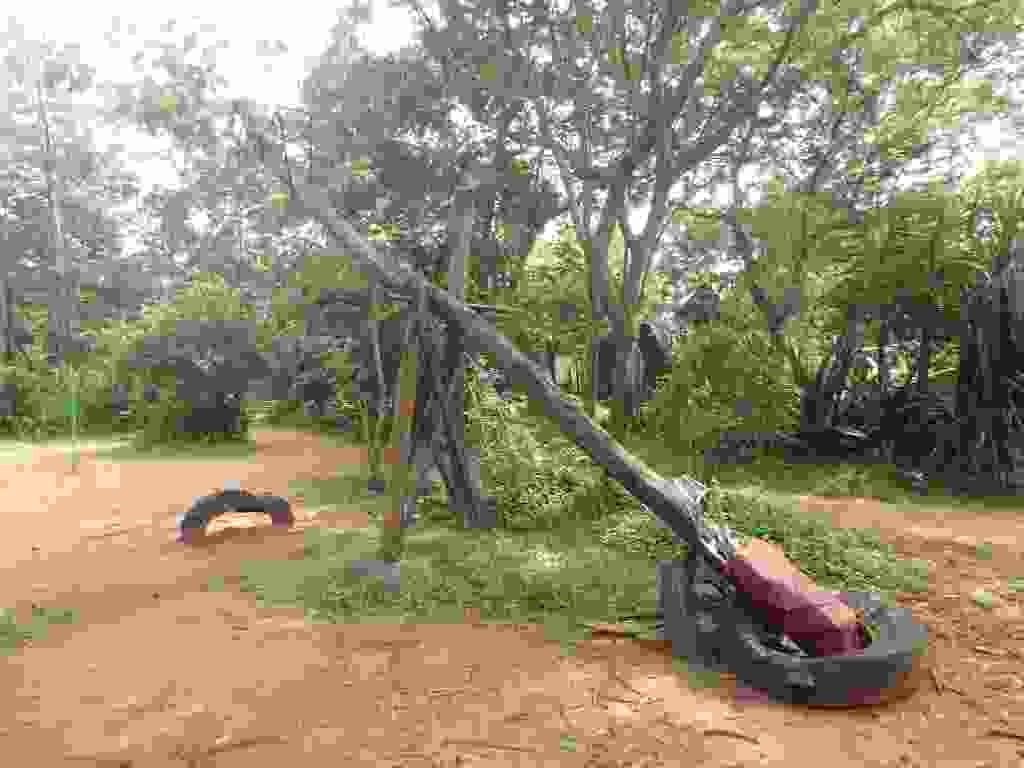
\includegraphics[width=\mywidth]{../wp-content/uploads/2015/12/wpid-oi000605-1024x768.jpg} \end{center}

 Et des volontaires viennent travailler et apprendre pour des durées de quelques jours à plusieurs mois : entretien du lieu, constructions en bois, cuisine... L'organisation est très libre et très peu d'argent est utilisé. 

 Marché le samedi matin. 
\begin{center} 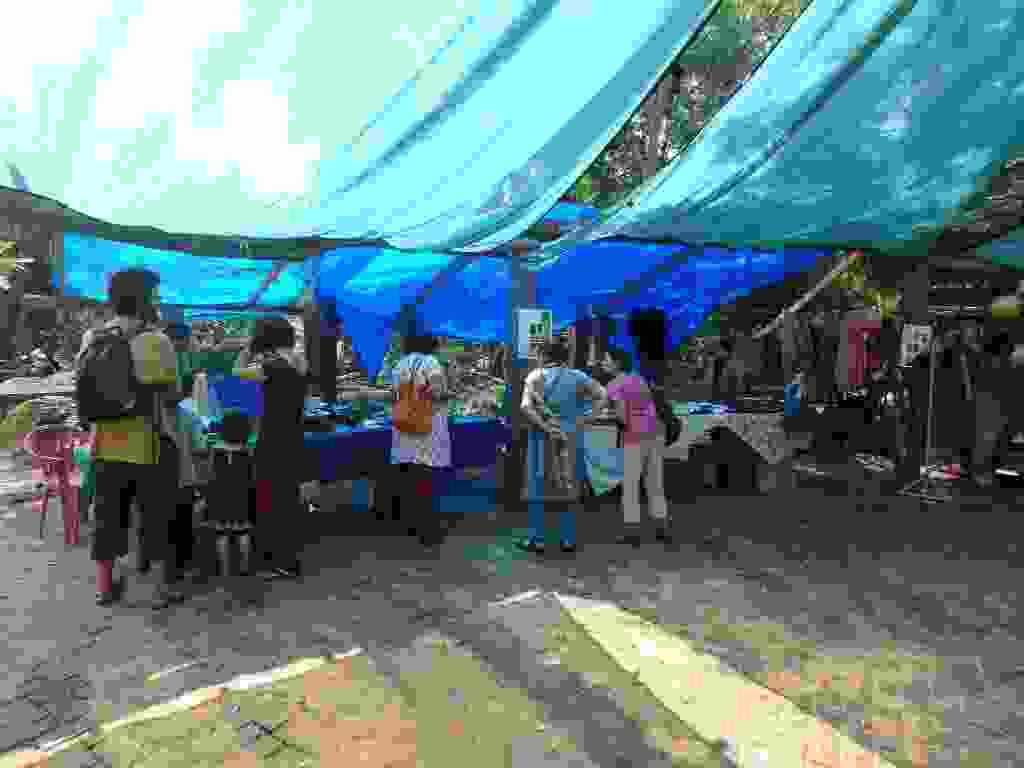
\includegraphics[width=\mywidth]{../wp-content/uploads/2015/12/wpid-oi000627-1024x768.jpg} \end{center}

\pagebreak
 Préparation des dosas. 
\begin{center} 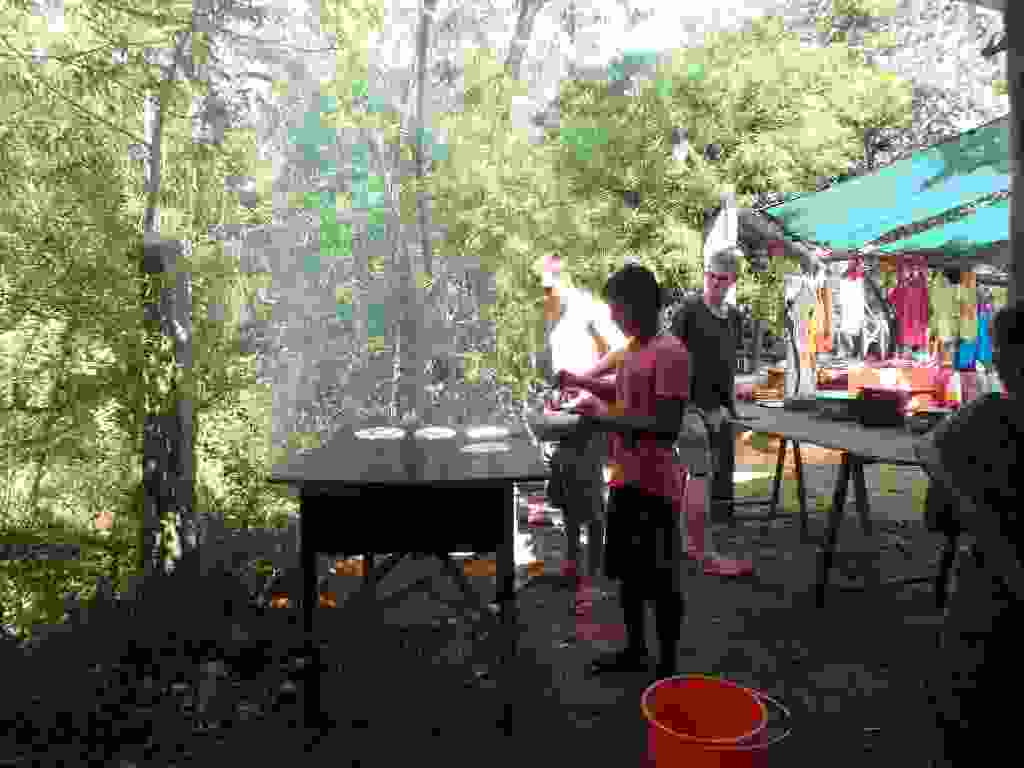
\includegraphics[width=\mywidth]{../wp-content/uploads/2015/12/wpid-oi0006291-1024x768.jpg} \end{center}

  Cuisine pour la soirée pizzas. 
\begin{center} 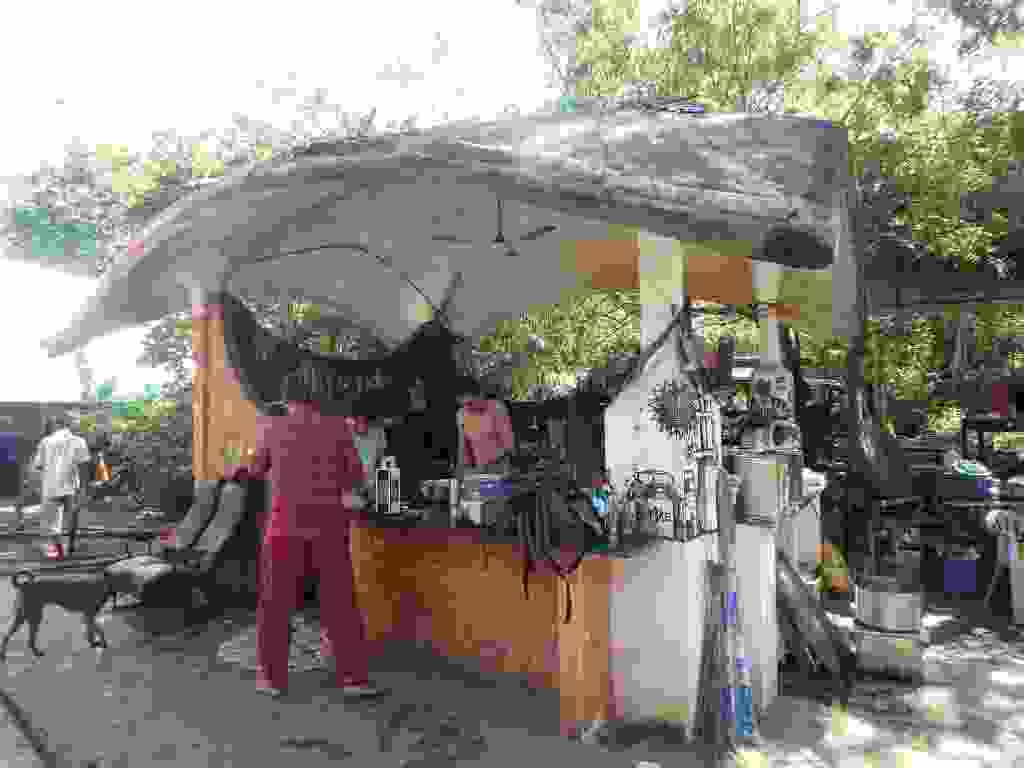
\includegraphics[width=\mywidth]{../wp-content/uploads/2015/12/wpid-oi0006241-1024x768.jpg} \end{center}

  J'ai visité d'autres communautés : 

 Sadhana forest : le projet est la reforestation et la préservation de l'eau. Organisation stricte avec beaucoup de règles : alcool, tabac et drogues interdits, nourriture vegane, économie des ressources maximale. La visite était gratuite avec projection d'un film et repas offert. 
\begin{center} 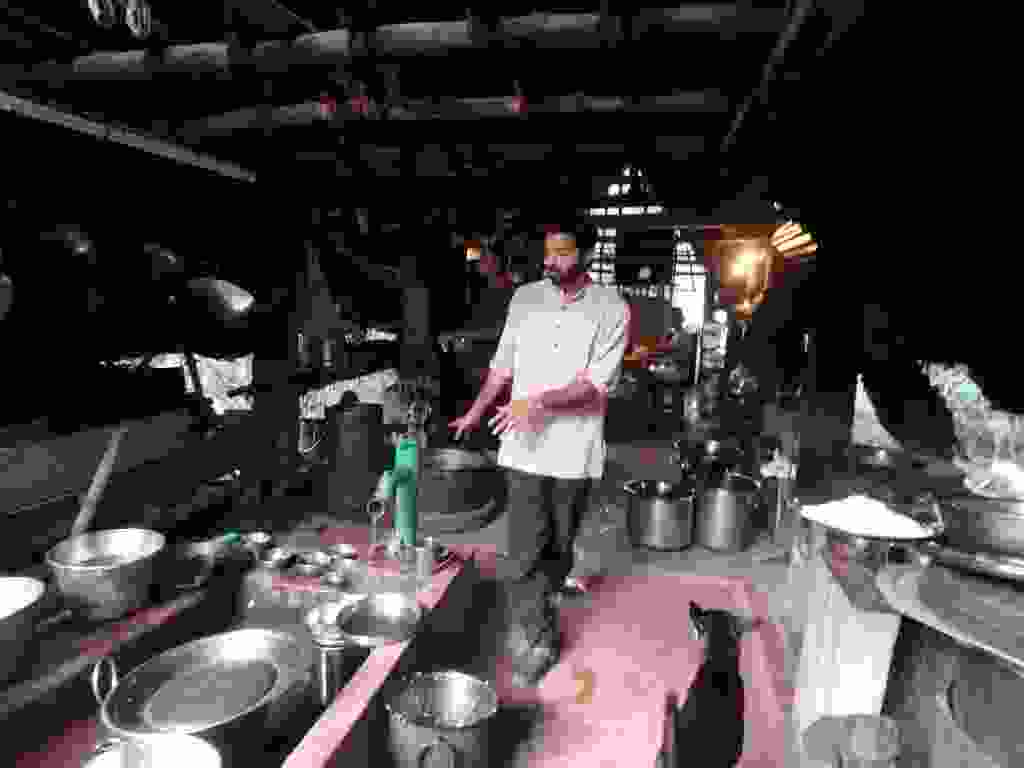
\includegraphics[width=\mywidth]{../wp-content/uploads/2015/12/wpid-oi000616-1024x768.jpg} \end{center}

 Électricité fournie par des panneaux solaires...
\begin{center} 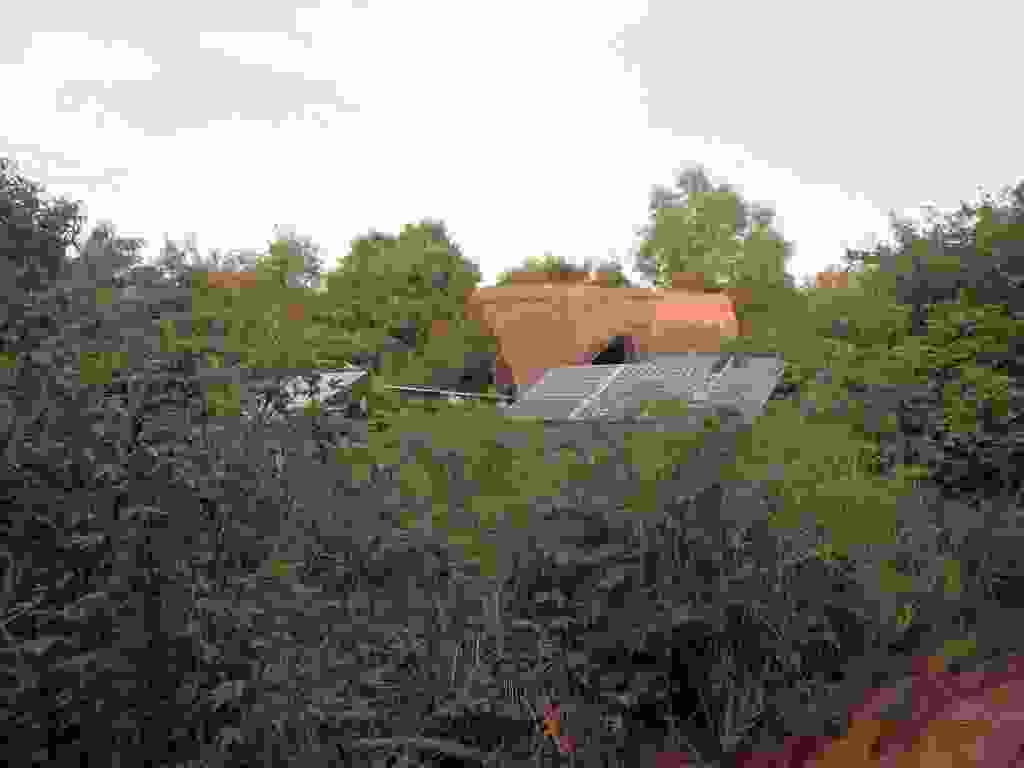
\includegraphics[width=\mywidth]{../wp-content/uploads/2015/12/wpid-oi000617-1024x768.jpg} \end{center}

\pagebreak
 ...ou des vélos s'il ne fait pas beau. 
\begin{center} 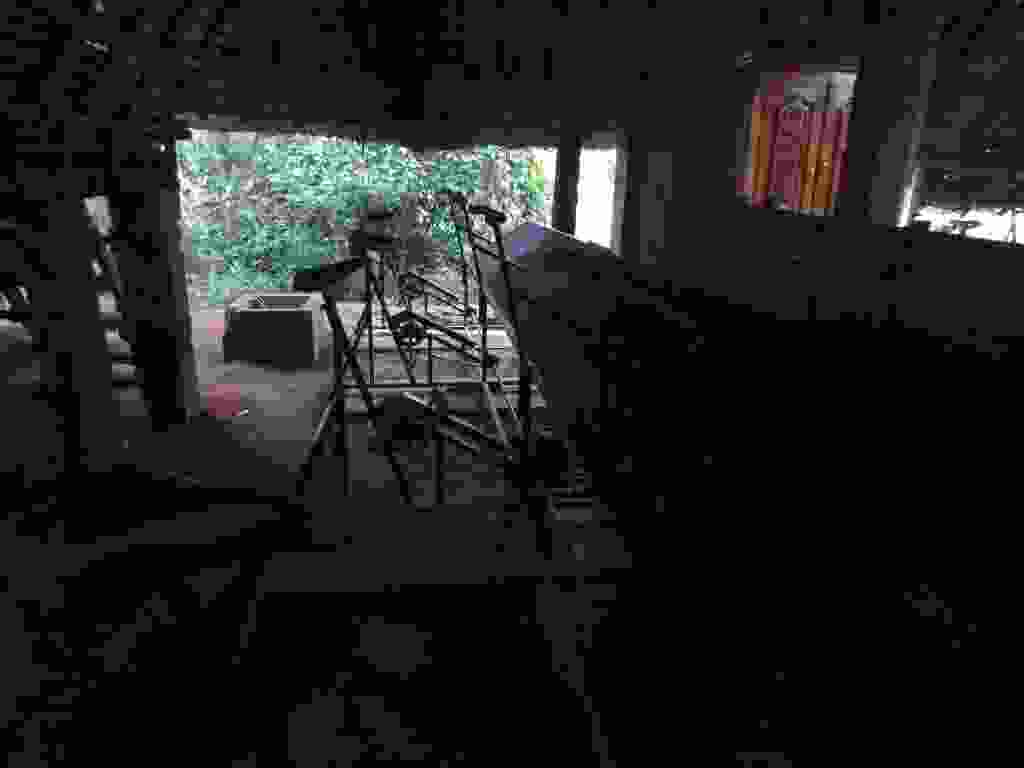
\includegraphics[width=\mywidth]{../wp-content/uploads/2015/12/wpid-oi000620-1024x768.jpg} \end{center}

 Vélo pour faire tourner un mixeur. 
\begin{center} 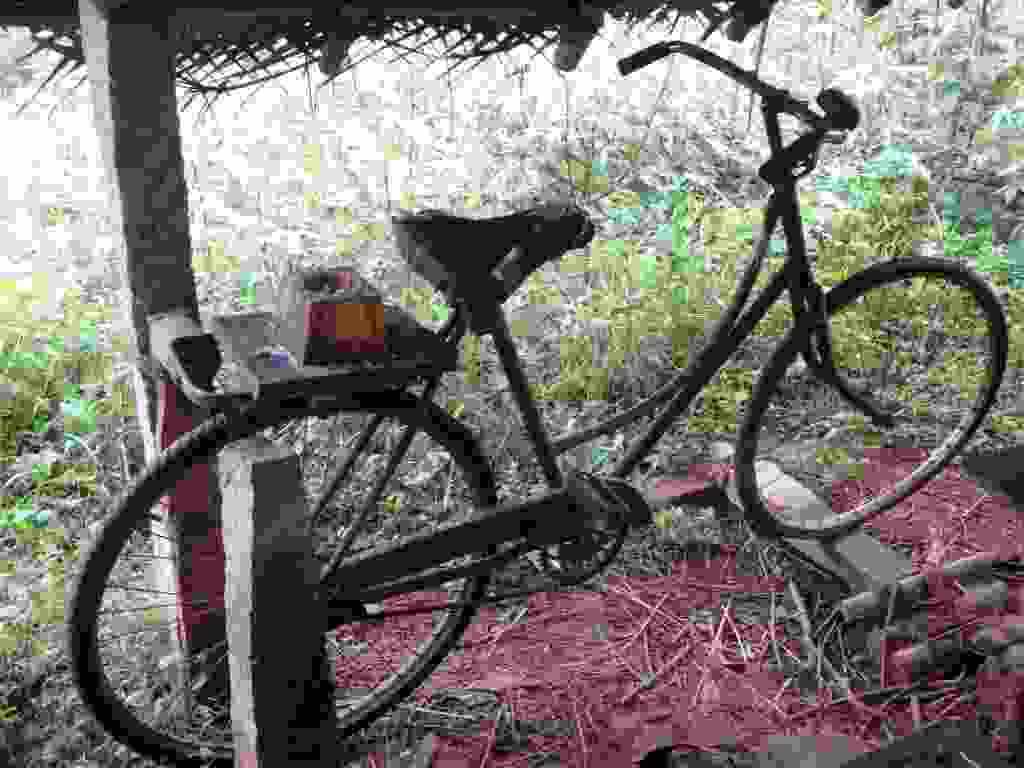
\includegraphics[width=\mywidth]{../wp-content/uploads/2015/12/wpid-oi000619-1024x768.jpg} \end{center}

\pagebreak
 Vaisselle faite avec de la cendre. 
\begin{center} 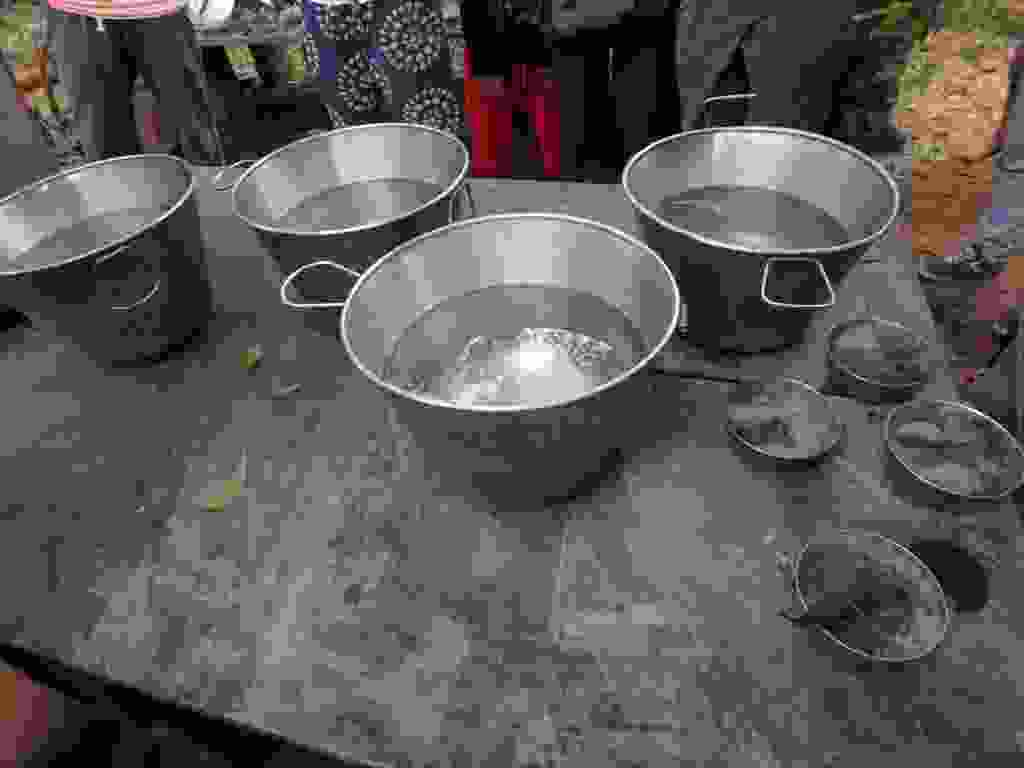
\includegraphics[width=\mywidth]{../wp-content/uploads/2015/12/wpid-oi000621-1024x768.jpg} \end{center}

 J'ai passé 1/2 journée à aider à la construction de maisons en argile et paille dans la communauté Sacred Grove. Une trentaine d'étudiants architectes indiens étaient volontaires ici. 
\begin{center} 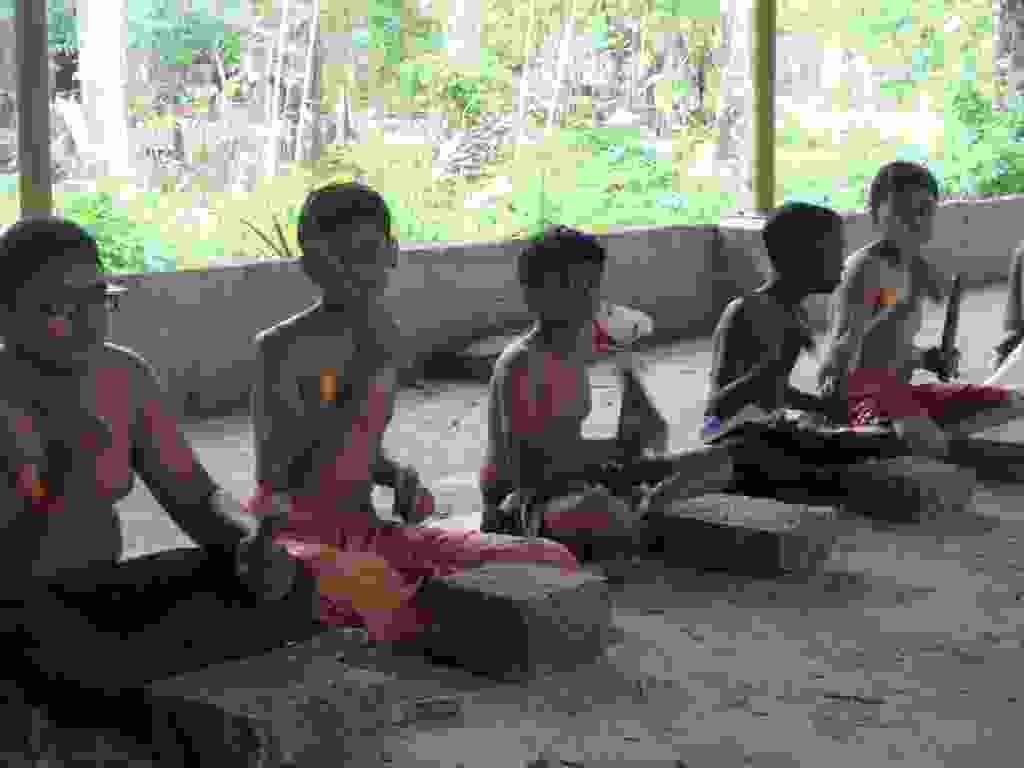
\includegraphics[width=\mywidth]{../wp-content/uploads/2015/12/wpid-oi000267-1024x768.jpg} \end{center}
\begin{center} 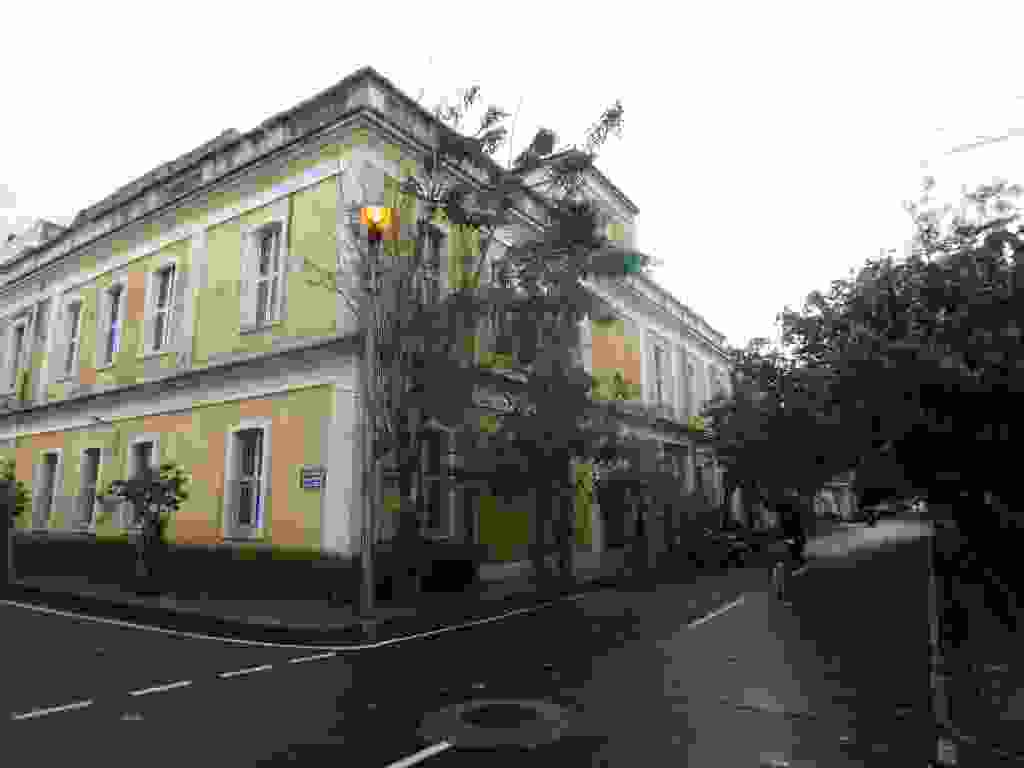
\includegraphics[width=\mywidth]{../wp-content/uploads/2015/12/wpid-oi000554-1024x768.jpg} \end{center}
\begin{center} 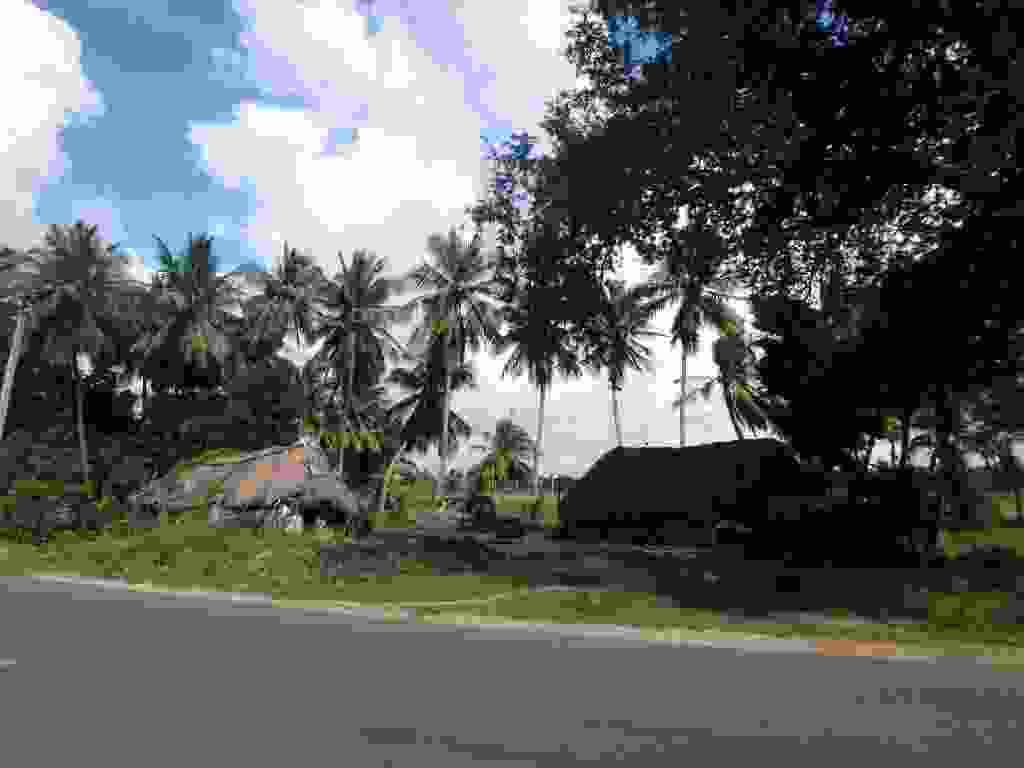
\includegraphics[width=\mywidth]{../wp-content/uploads/2015/12/wpid-oi000546-1024x768.jpg} \end{center}
\begin{center} 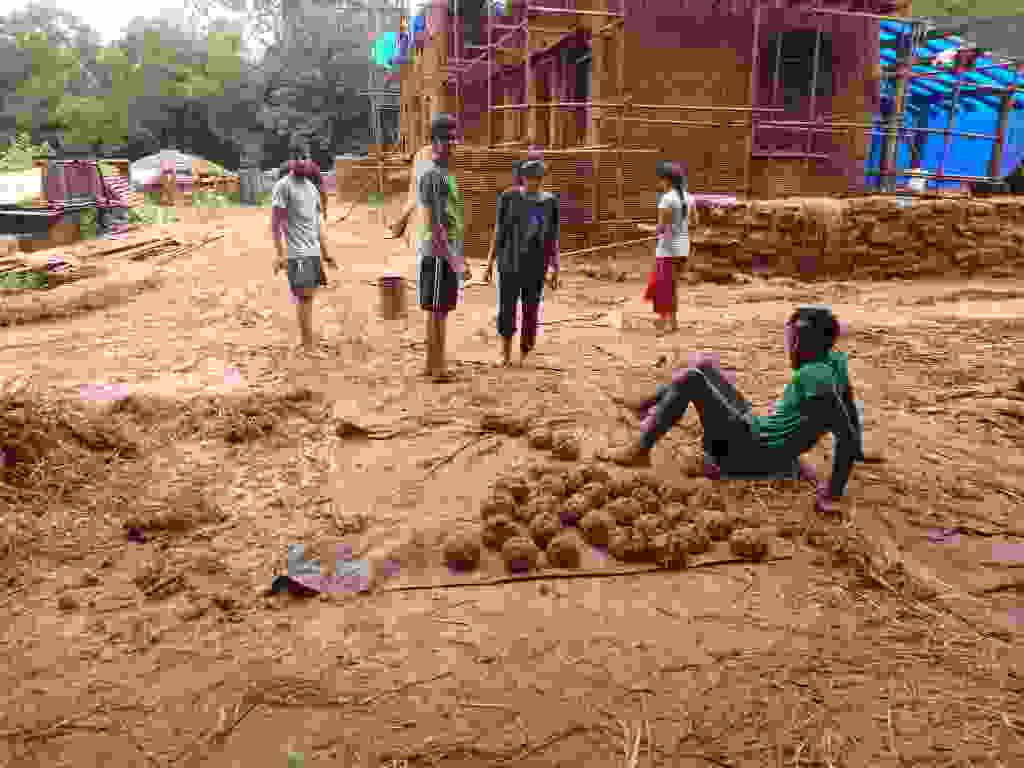
\includegraphics[width=\mywidth]{../wp-content/uploads/2015/12/wpid-oi000552-1024x768.jpg} \end{center}

 Visite de Solitude, restaurant et ferme en permaculture et agriculture naturelle : riz, millet, fruits et légumes. Après 4 jours de pluie non stop, il n'y avait pas beaucoup d'activité. 
\begin{center} 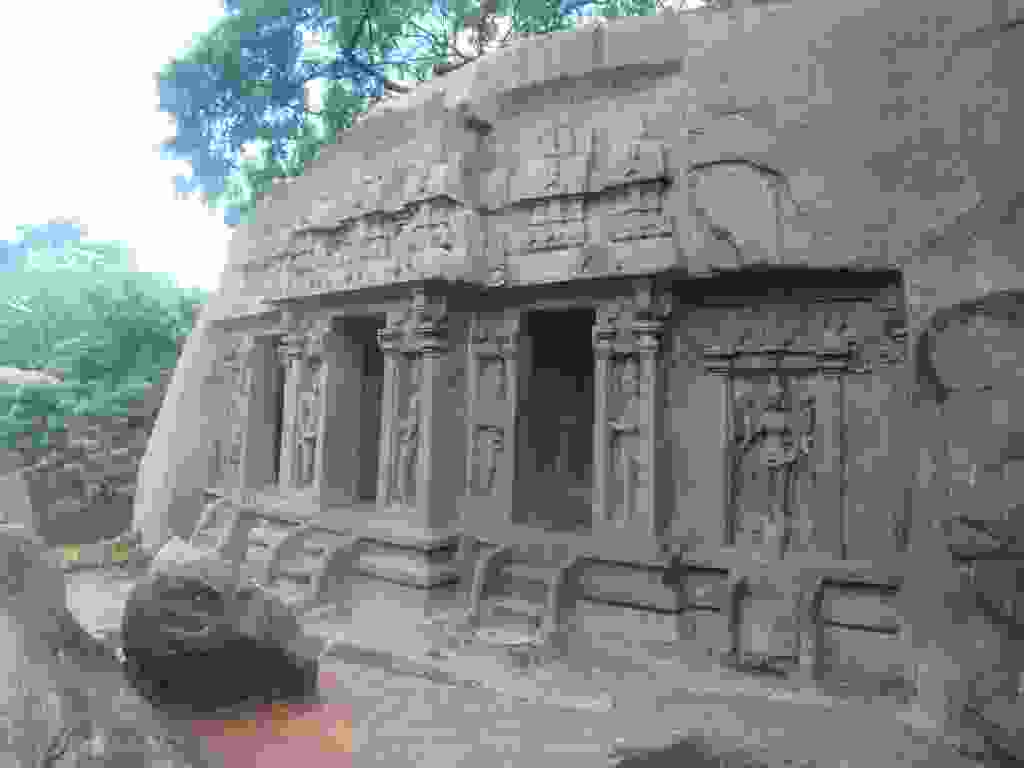
\includegraphics[width=\mywidth]{../wp-content/uploads/2015/12/wpid-oi000590-1024x768.jpg} \end{center}
\begin{center} 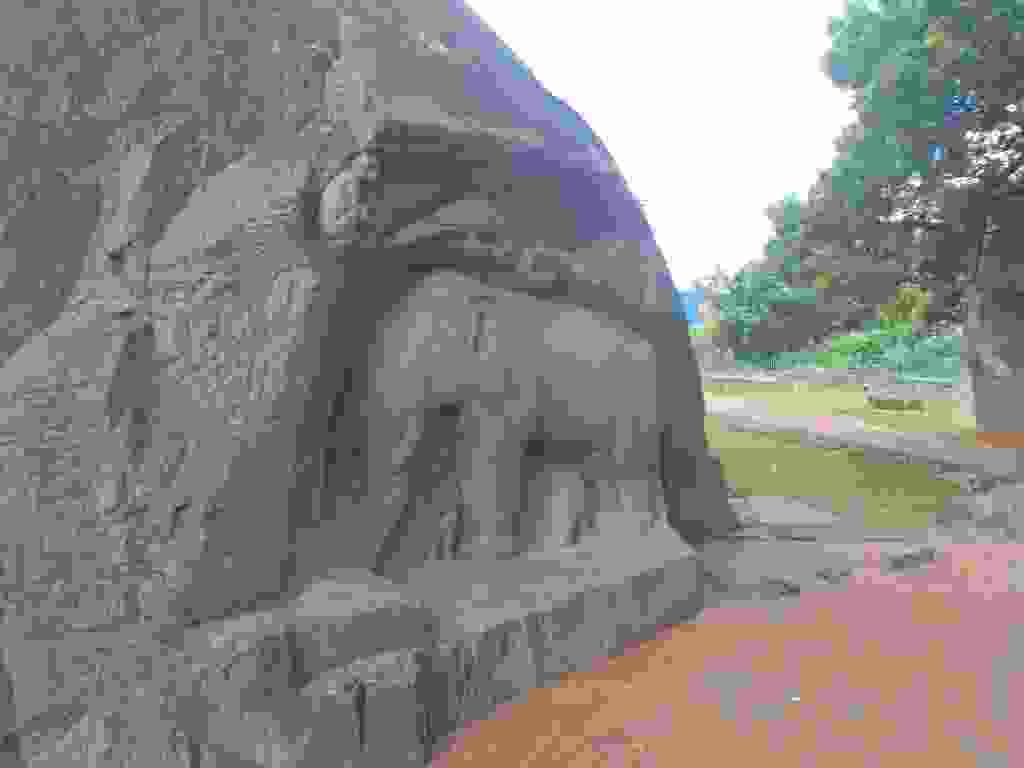
\includegraphics[width=\mywidth]{../wp-content/uploads/2015/12/wpid-oi000593-1024x768.jpg} \end{center}
\begin{center} 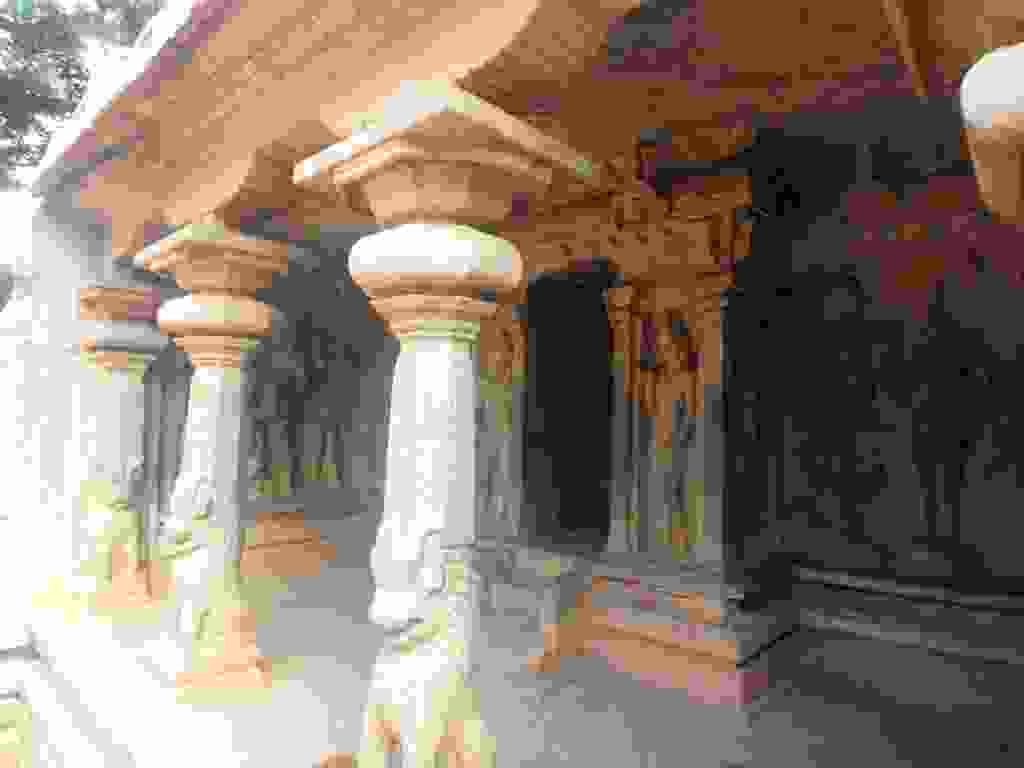
\includegraphics[width=\mywidth]{../wp-content/uploads/2015/12/wpid-oi000587-1024x768.jpg} \end{center}
